% =====================================================================
%  ncwu_beamer_defense_red
%  来源：红色通用毕业答辩模板（原 30 页）（YangTex 模板库 · 用户原稿全量保留版）
%  处理：仅删除编译产物 PDF / digest.lock，把 \input 递归展开为单文件；
%        正文、章节、例题、每张幻灯片、封面与参考文献一字未改。
%  字体：原稿的 macOS 字体声明全部保留，外加 \IfFontExistsTF 存在性判断；
%        在 Mac 上视觉与原 PDF 完全一致，在 Windows / Linux 上字体缺失时
%        自动跳过该声明改用默认字体，仍能正常编译。
%  编译：xelatex（目录 / 交叉引用需连续编译 2~3 遍，产品已自动处理）
% =====================================================================

% !TEX TS-program = xelatex
% =====================================================================
%  红色通用毕业答辩模板 —— LaTeX/Beamer 复刻优化版
%  复刻自《红色通用毕业答辩模板.pptx》(30 页)，全部插图由 TikZ 绘制，
%  不依赖任何外部图片文件，单文件即可编译。
%
%  编译方式：xelatex 编译两遍（推荐 latexmk -xelatex）
%  字体说明：macOS 使用 fontset=mac；Windows 请改为 fontset=windows；
%            Linux 请改为 fontset=fandol（或 ubuntu）。
%  内容替换：搜索「答辩人」「指导教师」「课题名称」等标记处即可替换。
% =====================================================================
\documentclass[aspectratio=169,11pt]{beamer}
\usepackage[UTF8]{ctex}          % 换平台时修改 fontset
\usepackage{amsmath,amssymb}
% --------- 西文字体：Times New Roman（正文、无衬线、等宽统一） ---------
\usepackage{newtxmath}                       % 数学字体与 Times 协调
\IfFontExistsTF{Times New Roman}{\setmainfont{Times New Roman}[BoldFont={Times New Roman Bold},
  ItalicFont={Times New Roman Italic},BoldItalicFont={Times New Roman Bold Italic}]}{}
\IfFontExistsTF{Times New Roman}{\setsansfont{Times New Roman}[BoldFont={Times New Roman Bold},
  ItalicFont={Times New Roman Italic},BoldItalicFont={Times New Roman Bold Italic}]}{}
\IfFontExistsTF{Menlo}{\setmonofont{Menlo}}{}
\usepackage{tikz}
\usetikzlibrary{arrows.meta,backgrounds,calc,chains,decorations.pathreplacing,
                fit,matrix,patterns.meta,positioning,shadows,shapes.geometric,
                shapes.misc,shapes.symbols}
\usepackage{pgfplots}
\pgfplotsset{compat=1.18}
\usepackage{booktabs,array,multirow}

% ------------------------- 配色体系 -------------------------
\definecolor{crimson}{HTML}{9E1B1B}      % 主色：中国红
\definecolor{crimsonL}{HTML}{C8383C}     % 亮红
\definecolor{crimsonD}{HTML}{6C0F13}     % 深红（封面/过渡页渐变）
\definecolor{gold}{HTML}{C9A45B}         % 金色点缀
\definecolor{ink}{HTML}{2A2A2C}          % 正文墨色
\definecolor{grayt}{HTML}{7C7C82}        % 次级灰字
\definecolor{paperbg}{HTML}{FBF8F5}      % 页面底色（宣纸白）
\definecolor{linegray}{HTML}{E6DFD6}     % 分隔线
\definecolor{softbg}{HTML}{F6EFEA}       % 卡片底色
\definecolor{blueaux}{HTML}{2F5D7C}      % 辅助色（对比用）

% ------------------------- 中文字族 -------------------------
\IfFontExistsTF{PingFang SC}{\setCJKfamilyfont{heiti}{PingFang SC}}{\setCJKfamilyfont{heiti}{FandolHei}}
\newcommand{\cnhei}{\CJKfamily{heiti}}    % 用于标题/强调（声明式，可进 font=）
\newcommand{\hei}[1]{{\cnhei#1}}

% ------------------------- Beamer 主题 -------------------------
\setbeamersize{text margin left=1cm,text margin right=1cm}
\setbeamercolor{normal text}{fg=ink,bg=paperbg}
\setbeamercolor{frametitle}{fg=ink}
\setbeamercolor{footline}{fg=grayt}
\setbeamercolor{structure}{fg=crimson}
\setbeamercolor{item}{fg=crimson}
\setbeamercolor{enumerate item}{fg=crimson}
\setbeamercolor{block title}{fg=white,bg=crimson}
\setbeamercolor{block body}{fg=ink,bg=softbg}
\setbeamertemplate{navigation symbols}{}
\setbeamertemplate{headline}{}
\setbeamertemplate{itemize items}[circle]
\setbeamertemplate{enumerate items}[default]
\setbeamertemplate{blocks}[rounded][shadow=false]
\setbeamertemplate{background canvas}{%
  \begin{tikzpicture}[remember picture,overlay]
    \fill[paperbg] (current page.south west) rectangle (current page.north east);
  \end{tikzpicture}}
% 内容页背景装饰：右上斜角 + 右下同心弧 + 左下点阵
\setbeamertemplate{background}{%
  \begin{tikzpicture}[remember picture,overlay]
    \fill[crimson!12] (current page.north east) -- ++(-1.5,0) -- ++(0,-1.5) -- cycle;
    \foreach \r in {1.9,2.7,3.5}{%
      \draw[crimson!10,line width=0.7pt]
        ([xshift=-0.7cm,yshift=0.7cm]current page.south east) circle (\r);}
    \foreach \i in {0,...,13}{%
      \fill[crimson!16] ($(current page.south west)+(0.95+0.34*\i,-0.28)$) circle (0.022);}
  \end{tikzpicture}}

% ------------------------- 页眉（标题区） -------------------------
\makeatletter
\setbeamertemplate{frametitle}{%
  \vspace*{0.3cm}%
  \noindent\hspace{0.6cm}%
  \begin{minipage}[b]{\dimexpr\textwidth-0.6cm\relax}%
    % 红色竖条：内联规则，与标题文字同基线、等高 -> 天然垂直居中
    \color{crimson}\raisebox{-0.11cm}{\rule{0.1cm}{0.5cm}}\hspace{0.22cm}%
    \begin{minipage}[b]{0.55\textwidth}%
      {\cnhei\large\color{ink}\insertframetitle}%
    \end{minipage}\hfill%
    \begin{minipage}[b]{0.34\textwidth}%
      \raggedleft{\color{grayt}\scriptsize\itshape\insertframesubtitle}%
    \end{minipage}%
  \end{minipage}%
  \par\vspace{0.12cm}%
  \begin{tikzpicture}[remember picture,overlay]
    \draw[linegray,line width=0.6pt]
      ([xshift=1cm,yshift=-1.28cm]current page.north west) -- ++(\textwidth,0);
    \fill[gold] ([xshift=1cm,yshift=-1.28cm]current page.north west)
      rectangle ++(2.2cm,-1pt);
  \end{tikzpicture}%
  \vspace{0.16cm}}
% ------------------------- 页脚（章节名 + 进度条 + 页码） -------------------------
\setbeamertemplate{footline}{%
  \begin{beamercolorbox}[wd=\paperwidth,ht=0.72cm,dp=0.18cm,
                          leftskip=1cm,rightskip=1cm]{footline}
    \vspace{0.08cm}{\cnhei\footnotesize\color{crimson}\insertsectionhead}
    \hfill{\color{grayt}\scriptsize\insertframenumber\,/\,\inserttotalframenumber}
  \end{beamercolorbox}%
  \begin{tikzpicture}[remember picture,overlay]
    \pgfmathsetmacro{\prog}{\insertframenumber/\inserttotalframenumber}
    \draw[linegray,line width=1.3pt]
      ([xshift=1cm,yshift=0.13cm]current page.south west) -- ++(3.2cm,0);
    \draw[crimson,line width=1.3pt]
      ([xshift=1cm,yshift=0.13cm]current page.south west) -- ++(3.2*\prog cm,0);
  \end{tikzpicture}}
\makeatother
\makeatletter
% 内容页画布：原点 = 页面左上 + (1cm, -2.25cm)，y 向下为负，不占排版空间
\newenvironment{pagetikz}{\begin{tikzpicture}[remember picture,overlay,
    shift={($(current page.north west)+(1cm,-1.95cm)$)},x=1cm,y=1cm]}{\end{tikzpicture}}
\makeatother

% ===================== TikZ 图标（全部手绘，存为 box） =====================
\newsavebox{\icBook}
\begin{lrbox}{\icBook}
\begin{tikzpicture}[scale=0.5]
  \draw[crimson,line width=0.9pt] (0,0.35)--(2.4,0.35);
  \draw[crimson,line width=0.9pt] (0.1,0.35) to[out=270,in=180] (0.35,0.05)--(1.2,0.05)
    to[out=0,in=270] (1.35,0.35);
  \draw[crimson,line width=0.9pt] (1.2,0.35) to[out=270,in=180] (1.45,0.05)--(2.3,0.05)
    to[out=0,in=270] (2.45,0.35);
  \draw[crimson,line width=0.7pt] (0.9,0.35)--(0.9,0.05);
\end{tikzpicture}\end{lrbox}

\newsavebox{\icGear}
\begin{lrbox}{\icGear}
\begin{tikzpicture}[scale=0.5]
  \draw[crimson,line width=0.9pt] (0,0) circle (0.55);
  \foreach \a in {0,45,...,315}{%
    \draw[crimson,line width=0.9pt] (\a:0.55)--(\a:0.95);
    \fill[crimson] (\a:0.95) circle (0.09);}
  \fill[white] (0,0) circle (0.22);
  \draw[crimson,line width=0.9pt] (0,0) circle (0.22);
\end{tikzpicture}\end{lrbox}

\newsavebox{\icChart}
\begin{lrbox}{\icChart}
\begin{tikzpicture}[scale=0.5]
  \draw[crimson,line width=1pt] (0,0)--(2.6,0);
  \fill[crimson] (0.25,0) rectangle (0.75,0.75);
  \fill[crimsonL] (1.0,0) rectangle (1.5,1.45);
  \fill[gold] (1.75,0) rectangle (2.25,1.05);
  \draw[crimson,line width=0.8pt] (0,0)--(0,1.75);
\end{tikzpicture}\end{lrbox}

\newsavebox{\icTarget}
\begin{lrbox}{\icTarget}
\begin{tikzpicture}[scale=0.5]
  \draw[crimson,line width=0.9pt] (0,0) circle (1.05);
  \draw[crimsonL,line width=0.9pt] (0,0) circle (0.7);
  \fill[crimson] (0,0) circle (0.3);
  \draw[crimson,line width=0.8pt] (1.3,0)--(1.85,0);
  \draw[crimson,line width=0.8pt] (0,1.3)--(0,1.85);
\end{tikzpicture}\end{lrbox}

\newsavebox{\icFunc}
\begin{lrbox}{\icFunc}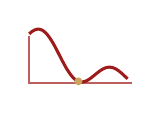
\begin{tikzpicture}[scale=0.5]
  \draw[crimson!70,line width=0.7pt] (0,1.2)--(0,0)--(2.6,0);
  \draw[crimson,line width=1.1pt,domain=0:2.5,samples=60] plot (\x,{0.15+1.1*exp(-1.3*\x*\x)+0.25*sin(220*\x)});
  \fill[gold] (1.25,{0.15+1.1*exp(-1.3*1.25*1.25)+0.25*sin(275)}) circle (0.1);
\end{tikzpicture}\end{lrbox}

\newsavebox{\icNet}
\begin{lrbox}{\icNet}
\begin{tikzpicture}[scale=0.5]
  \foreach \p/\q in {0.25/0.15,2.2/0.35,1.2/1.25,0.5/1.6,2.1/1.5}{%
    \fill[crimson] (\p,\q) circle (0.16);}
  \draw[crimsonL,line width=0.7pt] (0.25,0.15)--(1.2,1.25)--(2.2,0.35)
    --(0.5,1.6)--(2.1,1.5)--(1.2,1.25)--(0.5,1.6);
\end{tikzpicture}\end{lrbox}

\newsavebox{\icFlask}
\begin{lrbox}{\icFlask}
\begin{tikzpicture}[scale=0.5]
  \draw[crimson,line width=1pt] (0.95,1.75)--(0.95,0.75)--(0.25,0)--(2.05,0)--(1.35,0.75)--(1.35,1.75)--cycle;
  \fill[crimson!25] (0.42,0.18)--(1.88,0.18)--(1.35,0.78)--(0.95,0.78)--cycle;
  \draw[crimson,line width=0.9pt] (0.75,1.75)--(1.55,1.75);
\end{tikzpicture}\end{lrbox}

\newsavebox{\icDoc}
\begin{lrbox}{\icDoc}
\begin{tikzpicture}[scale=0.5]
  \draw[crimson,line width=1pt] (0.3,0)--(1.85,0)--(2.3,0.5)--(2.3,2.1)--(0.3,2.1)--cycle;
  \draw[crimson,line width=0.9pt] (1.85,0)--(1.85,0.5)--(2.3,0.5);
  \foreach \y in {0.85,1.2,1.55}{%
    \draw[crimsonL,line width=0.7pt] (0.6,\y)--(1.95,\y);}
\end{tikzpicture}\end{lrbox}

\newsavebox{\icStar}
\begin{lrbox}{\icStar}
\begin{tikzpicture}[scale=0.5]
  \draw[gold,line width=0.9pt,fill=gold!25]
    (90:1.05) \foreach \a in {162,234,306,18}{-- (\a:1.05)} -- cycle;
  \fill[crimson] (90:0.42) circle (0.12);
\end{tikzpicture}\end{lrbox}

\newsavebox{\icBulb}
\begin{lrbox}{\icBulb}
\begin{tikzpicture}[scale=0.5]
  \draw[crimson,line width=1pt] (0,1.15) circle (0.72);
  \draw[crimson,line width=0.9pt] (-0.35,0.5)--(0.35,0.5);
  \draw[crimson,line width=0.9pt] (-0.3,0.28)--(0.3,0.28);
  \draw[gold,line width=0.9pt] (-0.2,0.05)--(0.2,0.05);
  \fill[gold!40] (0,0.85) circle (0.28);
\end{tikzpicture}\end{lrbox}

% 图标输出宏（供 \foreach 中间接调用，\usebox 不能直接吃循环变量）
\newcommand{\icBookOut}{\scalebox{0.6}{\usebox{\icBook}}}
\newcommand{\icGearOut}{\scalebox{0.6}{\usebox{\icGear}}}
\newcommand{\icChartOut}{\scalebox{0.6}{\usebox{\icChart}}}
\newcommand{\icTargetOut}{\scalebox{0.6}{\usebox{\icTarget}}}
\newcommand{\icFuncOut}{\scalebox{0.6}{\usebox{\icFunc}}}
\newcommand{\icNetOut}{\scalebox{0.6}{\usebox{\icNet}}}
\newcommand{\icFlaskOut}{\scalebox{0.6}{\usebox{\icFlask}}}
\newcommand{\icDocOut}{\scalebox{0.6}{\usebox{\icDoc}}}
\newcommand{\icStarOut}{\scalebox{0.6}{\usebox{\icStar}}}
\newcommand{\icBulbOut}{\scalebox{0.6}{\usebox{\icBulb}}}

% ===================== 常用小构件（正文段落内可直接调用） =====================
% 圆形编号徽章
\newcommand{\numtag}[1]{%
  \tikz[baseline=-3pt]{\node[fill=crimson,text=white,circle,inner sep=0pt,
    font=\cnhei\scriptsize,minimum size=0.44cm]{#1};}}
% 方形大编号（过渡/卡片用）
\newcommand{\bignum}[1]{\scalebox{1}{\ hei{#1}\ }}
% 关键词标签（注意：内部含 tikz，仅用于正文，不能写在 pagetikz 画布内）
\newcommand{\kw}[1]{%
  \tikz[baseline=-3pt]{\node[draw=crimson,text=crimson,rounded corners=2pt,
    inner sep=3pt,font=\hei{\scriptsize}]{#1};}}
% 实心关键词标签
\newcommand{\kwf}[1]{%
  \tikz[baseline=-3pt]{\node[fill=crimson,text=white,rounded corners=2pt,
    inner sep=3pt,font=\hei{\scriptsize}]{#1};}}
% 带左侧红条的小标题
\newcommand{\subhead}[1]{%
  \par\vspace{2pt}\noindent
  \tikz[baseline=-2pt]{\fill[crimson] (0,0.22) rectangle (0.07,0.5);}%
  \hspace{4pt}{\cnhei\small\color{crimson}#1}\par\vspace{2pt}}

% ===================== 封面 =====================
\newcommand{\makecover}{%
\begingroup
\setbeamertemplate{frametitle}{}
\setbeamertemplate{background}{}
\setbeamertemplate{footline}{}
\setbeamertemplate{background canvas}{%
  \begin{tikzpicture}[remember picture,overlay]
    \fill[left color=crimsonD,right color=crimson] (current page.south west)
      rectangle (current page.north east);
    \fill[white,opacity=0.045] ([xshift=7.5cm]current page.south west)
      rectangle (current page.north east);
    \foreach \r in {2.4,3.3,4.2,5.1}{%
      \draw[white,opacity=0.09,line width=0.8pt]
        ([xshift=-1.6cm,yshift=1.4cm]current page.south east) circle (\r);}
    \foreach \i in {0,...,11}{%
      \fill[white,opacity=0.13] ($(current page.north east)+(-0.9-0.4*\i,-1.15)$) circle (0.026);
      \fill[white,opacity=0.09] ($(current page.north east)+(-0.9-0.4*\i,-1.45)$) circle (0.026);}
    \fill[gold,opacity=0.85] ([xshift=1cm,yshift=-1.55cm]current page.north west)
      rectangle ++(3.4cm,0.8pt);
    \fill[crimsonD!80] (current page.south west) rectangle ++(\paperwidth,0.35cm);
    \fill[gold,opacity=0.5] (current page.south west) rectangle ++(\paperwidth,0.06cm);
  \end{tikzpicture}}
\begin{frame}[plain]
\begin{tikzpicture}[remember picture,overlay]
  % 顶部信息
  \node[anchor=north west,text=white,font=\cnhei\large]
    at ([xshift=1cm,yshift=-0.85cm]current page.north west) {XX 大学 · 数学与统计学院};
  \node[anchor=north east,text=white!85,font=\hei{\small}]
    at ([xshift=-1cm,yshift=-0.9cm]current page.north east) {2026 届学位论文答辩};
  % 主标题
  \node[anchor=north west,text=white,text width=12.6cm,align=left,
        font=\fontsize{24}{30}\selectfont]
    at ([xshift=1cm,yshift=-2.4cm]current page.north west)
    {\hei{几类非线性发展方程解的爆破与整体存在性研究}};
  \node[anchor=north west,text=gold,text width=12.6cm,align=left,font=\fontsize{9.5}{12}\selectfont]
    at ([xshift=1.05cm,yshift=-5.1cm]current page.north west)
    {Blow-up and Global Existence of Solutions to Several Nonlinear Evolution Equations};
  \fill[gold] ([xshift=1.05cm,yshift=-6.35cm]current page.north west) rectangle ++(3.2cm,1pt);
  % 作者信息
  \node[anchor=south west,text=white,text width=8.5cm,align=left,
        font=\fontsize{11.5}{18}\selectfont]
    at ([xshift=1cm,yshift=1.05cm]current page.south west)
    {\cnhei 答辩人：XXX \quad 指导教师：XXX 教授\par
     \vspace{2pt}{\fontsize{9.5}{12}\selectfont 专\quad 业：基础数学 \quad 研究方向：偏微分方程}};
  \node[anchor=south east,text=white!85,align=right,font=\fontsize{10}{14}\selectfont]
    at ([xshift=-1cm,yshift=1.05cm]current page.south east)
    {2026 年 12 月};
\end{tikzpicture}
\end{frame}
\endgroup}

% ===================== 过渡页 =====================
% #1 编号 #2 部分名 #3 中文标题 #4 英文 #5 引言
\newcommand{\sectionframe}[5]{%
\begingroup
\setbeamertemplate{frametitle}{}
\setbeamertemplate{background}{}
\setbeamertemplate{footline}{}
\setbeamertemplate{background canvas}{%
  \begin{tikzpicture}[remember picture,overlay]
    \fill[left color=crimsonD,right color=crimson] (current page.south west)
      rectangle (current page.north east);
    \foreach \r in {2.0,2.9,3.8}{%
      \draw[white,opacity=0.10,line width=0.7pt]
        ([xshift=-1.1cm,yshift=1.1cm]current page.south east) circle (\r);}
    \foreach \i in {0,...,16}{%
      \fill[white,opacity=0.14] ($(current page.south west)+(0.55+0.42*\i,-0.3)$) circle (0.024);
      \fill[white,opacity=0.09] ($(current page.south west)+(0.55+0.42*\i,-0.5)$) circle (0.024);}
    \fill[white,opacity=0.07] ([xshift=-1.15cm]current page.north east)
      rectangle ++(0.14cm,-7.2cm);
  \end{tikzpicture}}
\begin{frame}[plain]
\begin{tikzpicture}[remember picture,overlay]
  % 超大半透明编号（居中水印）
  \node[anchor=center,text=white,opacity=0.13,
        font=\fontsize{150}{150}\selectfont]
    at (current page.center) {#1};
  % 部分名（金色，水平+垂直居中）
  \node[anchor=center,text=gold,font=\cnhei\Large,
        text width=14cm,align=center]
    at ([yshift=2.3cm]current page.center) {#2};
  % 金色短线（水平居中）
  \fill[gold] ($(current page.center)+(0,1.6cm)+(-1.3cm,0)$)
    rectangle ++(2.6cm,0.8pt);
  % 主标题（白色，居中）
  \node[anchor=center,text=white,text width=14cm,align=center,
        font=\fontsize{27}{33}\selectfont]
    at ([yshift=0.85cm]current page.center) {\hei{#3}};
  % 英文副标题（金色，居中）
  \node[anchor=center,text=gold!85,font=\fontsize{11}{13}\selectfont,
        text width=14cm,align=center]
    at ([yshift=-0.15cm]current page.center) {#4};
  % 引言文字（白色半透明，居中）
  \node[anchor=center,text=white!80,text width=11cm,align=center,
        font=\fontsize{9.5}{14}\selectfont]
    at ([yshift=-2.3cm]current page.center) {#5};
\end{tikzpicture}
\end{frame}
\endgroup}

% ===================== 文档正文 =====================
\begin{document}

\makecover

% ------------------------- 目录 -------------------------
\begin{frame}[t]{目录}{Contents}
\begin{pagetikz}
  \foreach \n/\xt/\yt/\cn/\en/\ic in
    {01/0/0/{研究背景与意义}/{Research Background and Significance}/\icBookOut,
     02/7.1/0/{理论框架与方法}/{Theoretical Framework and Methods}/\icGearOut,
     03/0/-2.6/{数值实验与结果}/{Numerical Experiments and Results}/\icChartOut,
     04/7.1/-2.6/{总结与展望}/{Conclusions and Future Work}/\icTargetOut}{%
    \draw[linegray,fill=white,rounded corners=2pt] (\xt,\yt) rectangle ++(6.5,-2.35);
    \fill[crimson] (\xt,\yt) rectangle ++(0.09,-2.35);
    \node[anchor=north west,text=crimson!28,font=\fontsize{25}{25}\selectfont]
      at (\xt+0.3,\yt-0.12) {\n};
    \node[anchor=north west,text=ink,font=\cnhei\large]
      at (\xt+1.35,\yt-0.25) {\cn};
    \node[anchor=north east] at (\xt+6.2,\yt-0.28) {\ic};
    \fill[gold] (\xt+0.3,\yt-1.28) rectangle ++(1.2cm,0.8pt);
    \node[anchor=north west,text=grayt,font=\fontsize{8.5}{10.5}\selectfont]
      at (\xt+0.3,\yt-1.52) {\en};
  }
\end{pagetikz}
\end{frame}

% ================= 第一部分：研究背景与意义 =================
\section{研究背景与意义}
\sectionframe{01}{第 一 部 分}{研究背景与意义}{Research Background and Significance}
{从物理模型出发，明确非线性发展方程中爆破现象的研究价值与本文拟解决的关键问题。}

% ---------- 第 4 页版式：两栏图文 + 底部方程条 ----------
\begin{frame}[t]{研究背景与问题提出}{Research Background and Motivation}
\begin{pagetikz}
  % 左卡片
  \draw[linegray,fill=white,rounded corners=2pt] (0,0) rectangle (6.65,-3.45);
  \fill[crimson] (0,0) rectangle (0.09,-3.45);
  \node[anchor=north west] at (0.32,-0.24) {\icNetOut};
  \node[anchor=north west,text=ink,font=\cnhei\small] at (1.75,-0.28) {物理与工程背景};
  \node[anchor=north west,text=grayt,text width=6.0cm,align=left,
        font=\fontsize{8.8}{12.4}\selectfont] at (0.32,-1.28)
    {非线性发展方程广泛出现于流体力学、等离子体物理、相场模型与图像处理等领域；可压缩磁流体力学（MHD）方程组刻画导电流体与磁场的耦合演化，其解的奇性形成机制与长时间行为长期是核心难点。};
  % 右卡片
  \draw[linegray,fill=white,rounded corners=2pt] (7.05,0) rectangle (13.7,-3.45);
  \fill[crimson] (7.05,0) rectangle (7.14,-3.45);
  \node[anchor=north west] at (7.37,-0.24) {\icTargetOut};
  \node[anchor=north west,text=ink,font=\cnhei\small] at (8.8,-0.28) {问题提出};
  \node[anchor=north west,text=grayt,text width=6.0cm,align=left,
        font=\fontsize{8.8}{12.4}\selectfont] at (7.37,-1.28)
    {对半线性抛物模型 $u_t-\Delta u=|u|^{p-1}u$，Fujita 临界指数 $p_F=1+\frac{2}{N}$ 决定了整体存在与有限时刻爆破的分野。本文关注临界与近临界情形下阻尼与非局部源如何改变爆破门槛。};
  % 底部方程条
  \fill[crimson] (0,-3.85) rectangle (13.7,-5.45);
  \fill[gold] (0,-3.85) rectangle (0.09,-5.45);
  \node[anchor=west,text=white,font=\cnhei\footnotesize] at (0.35,-4.15) {研究模型};
  \node[anchor=west,text=white,font=\fontsize{12}{14}\selectfont] at (1.8,-4.2)
    {$u_t-\Delta u+\mu(-\Delta)^{\alpha}u=|u|^{p-1}u,\quad (x,t)\in\mathbb{R}^N\times\mathbb{R}_+$};
  \node[anchor=west,text=white!85,font=\fontsize{8.8}{11}\selectfont] at (0.35,-4.95)
    {初值 $u_0\in H^1(\mathbb{R}^N)$，$p>1$，$\mu\ge 0$，$\alpha\in(0,1]$ 分别为阻尼强度与阻尼阶数。};
\end{pagetikz}
\end{frame}

% ---------- 第 5 页版式：四宫格（研究现状与不足） ----------
\begin{frame}[t]{国内外研究现状}{State of the Art}
\begin{pagetikz}
  \foreach \n/\x/\y/\ti/\te in
    {01/0/0/{经典理论与经典判据}/{Fujita 指数与 Levine 凸性方法已形成完整体系，为后续研究提供基准。\newline {\color{crimson!80}不足：}强依赖正初值与能量负性，适用范围受限。},
     02/7.05/0/{临界与近临界情形}/{$p=p_F$ 时爆破与整体存在同时出现，判据需要更精细刻画。\newline {\color{crimson!80}不足：}判据对初值形状高度敏感，缺少定量门槛。},
     03/0/-2.6/{非局部项与分数阶阻尼}/{记忆项与分数阶阻尼改变能量结构，解行为显著不同。\newline {\color{crimson!80}不足：}现有结论分散，缺少统一处理框架。},
     04/7.05/-2.6/{数值验证与算法实现}/{已有格式难以准确刻画爆破时刻与生命跨度。\newline {\color{crimson!80}不足：}高维临界问题的自适应验证仍不充分。}}{%
    \draw[linegray,fill=white,rounded corners=2pt] (\x,\y) rectangle ++(6.65,-2.35);
    \fill[crimson] (\x,\y) rectangle ++(0.09,-2.35);
    \node[anchor=north west,text=crimson!26,font=\fontsize{22}{22}\selectfont]
      at (\x+0.32,\y-0.12) {\n};
    \node[anchor=north west,text=ink,font=\cnhei\small] at (\x+1.35,\y-0.16) {\ti};
    \node[anchor=north west,text=grayt,text width=6.0cm,align=left,
          font=\fontsize{8.4}{11.6}\selectfont] at (\x+0.32,\y-0.72) {\te};
  }
\end{pagetikz}
\end{frame}

% ---------- 第 6 页版式：四步流程（技术路线） ----------
\begin{frame}[t]{技术路线}{Technical Roadmap}
\begin{pagetikz}
  \foreach \n/\x/\ti/\te in
    {01/0/{问题建模}/{建立带分数阶阻尼与非局部源的发展方程模型，明确初值空间与边界条件。},
     02/3.6/{理论分析}/{构造能量泛函与 Nehari 流形，证明局部适定性、爆破判据与生命跨度上界。},
     03/7.2/{数值验证}/{设计守恒型差分—谱混合格式，自适应逼近爆破时刻并验证收敛阶。},
     04/10.8/{总结提炼}/{对比理论门槛与数值结果，解释物理含义并给出方法适用边界。}}{%
    \draw[linegray,fill=white,rounded corners=2pt] (\x,0) rectangle ++(3.1,-4.3);
    \fill[crimson] (\x+0.55,-0.45) circle (0.25);
    \node[anchor=center,text=white,font=\cnhei\scriptsize] at (\x+0.55,-0.45) {\n};
    \node[anchor=north west,text=ink,font=\cnhei\small] at (\x+0.95,-0.24) {\ti};
    \node[anchor=north west,text=grayt,text width=2.65cm,align=left,
          font=\fontsize{8.2}{11.4}\selectfont] at (\x+0.25,-0.95) {\te};
  }
  \foreach \x in {3.25,6.85,10.45}{%
    \fill[crimsonL] (\x,-2.35)--(\x+0.28,-2.15)--(\x,-1.95)--cycle;}
\end{pagetikz}
\end{frame}


% ================= 第二部分：理论框架与方法 =================
\section{理论框架与方法}
\sectionframe{02}{第 二 部 分}{理论框架与方法}{Theoretical Framework and Methodology}
{以能量方法为主线，建立位势井结构与爆破判据，并给出严格的先验估计与存在性结果。}



% ---------- 第 9 页版式：四宫格方法卡片 ----------
\begin{frame}[t]{核心方法与数学工具}{Core Methods and Mathematical Tools}
\begin{pagetikz}
  \foreach \x/\y/\ic/\ti/\fm/\te in
    {0/0/\icFuncOut/{能量泛函}/{$\displaystyle E(u)=\frac{1}{2}\|\nabla u\|_2^2-\frac{1}{p+1}\|u\|_{p+1}^{p+1}$}/
      {刻画系统的守恒（耗散）结构，是判别解行为的第一工具。},
     7.05/0/\icTargetOut/{位势井与 Nehari 流形}/{$\displaystyle d=\inf_{u\in\mathcal{N}}E(u),\quad I(u)=\|\nabla u\|_2^2-\|u\|_{p+1}^{p+1}$}/
      {以井深 $d$ 为门槛，区分井内稳定解与井外不稳定解。},
     0/-2.6/\icBulbOut/{Levine 凸性方法}/{$\displaystyle E(u_0)<0\ \Longrightarrow\ T_{\max}<\infty$}/
      {由能量负性导出有限时刻爆破，并给出生命跨度上界估计。},
     7.05/-2.6/\icGearOut/{Galerkin 逼近}/{$\displaystyle u^m=\sum_{j=1}^{m}c_j^m(t)w_j(x)$}/
      {结合紧性方法取得弱解，为数值格式收敛性提供理论基础。}}{%
    \draw[linegray,fill=white,rounded corners=2pt] (\x,\y) rectangle ++(6.65,-2.35);
    \fill[crimson] (\x,\y) rectangle ++(0.09,-2.35);
    \node[anchor=north west] at (\x+0.32,\y-0.2) {\ic};
    \node[anchor=north west,text=ink,font=\cnhei\small] at (\x+1.45,\y-0.26) {\ti};
    \node[anchor=north west,text=crimson,font=\fontsize{9.5}{12}\selectfont]
      at (\x+1.5,\y-0.95) {\fm};
    \node[anchor=north west,text=grayt,text width=6.0cm,align=left,
          font=\fontsize{8.2}{11}\selectfont] at (\x+0.32,\y-1.72) {\te};
  }
\end{pagetikz}
\end{frame}

% ---------- 第 10 页版式：左侧位势井示意图 + 右侧两要点 ----------
\begin{frame}[t]{位势井结构与能量门槛}{Potential Well Structure}
\begin{pagetikz}
  % ---- 左：位势井示意 ----
  \draw[linegray,fill=white,rounded corners=2pt] (0,0) rectangle (7.3,-5.4);
  \node[anchor=north west,text=ink,font=\cnhei\small] at (0.3,-0.2) {位势井示意：$J(\lambda)$};
  \begin{scope}[shift={(0.9,-3.5)}]
    \clip (-0.5,-1.1) rectangle (5.95,2.45);
    \draw[grayt,line width=0.8pt,-{Stealth[length=2mm]}] (0,0) -- (5.85,0)
      node[below,font=\tiny] {$\lambda$};
    \draw[grayt,line width=0.8pt,-{Stealth[length=2mm]}] (0,-1.0) -- (0,2.35)
      node[left,font=\tiny] {$J$};
    % J(lambda)=lambda^2/2-lambda^4/4，横向缩放 3.0、纵向缩放 8.8
    \draw[crimson,line width=1.4pt,-{Stealth[length=2mm]},domain=0:1.5,samples=120]
      plot (\x,{8.8*(0.5*\x*\x - 0.25*\x*\x*\x*\x)});
    \fill[gold!45,opacity=0.5] (0,0) rectangle (4.24,2.2);
    \draw[dashed,grayt,line width=0.7pt] (0,2.2) -- (2.5,2.2);
    \node[left,text=crimson,font=\fontsize{8}{10}\selectfont] at (-0.05,2.2) {$d$};
    \fill[crimson] (3.0,2.2) circle (0.07);
    \node[right,text=crimson,font=\fontsize{7.5}{9}\selectfont] at (3.2,2.2) {$\lambda_*=1$};
    \fill[crimson] (4.24,0) circle (0.07);
    \node[below right,text=crimson,font=\fontsize{7.5}{9}\selectfont] at (4.24,0) {$\sqrt{2}$};
    \node[text=crimson!85,font=\hei{\tiny}] at (1.9,1.0) {井内（稳定）};
  \end{scope}
  \node[anchor=north west,text=ink!80,font=\fontsize{8.8}{11}\selectfont] at (0.4,-4.9)
    {$J(\lambda)=\dfrac{\lambda^2}{2}-\dfrac{\lambda^{p+1}}{p+1}$，井深 $d=J(\lambda_*)$};
  % ---- 右：两个要点 ----
  \foreach \y/\ic/\ti/\te in
    {0/{井内准则：整体存在}/\icTargetOut/{若 $E(u_0)<d$ 且 $I(u_0)>0$，则解整体存在且能量指数衰减：
      $\|u(t)\|_{H^1}\le C(1+t)^{-\frac{1}{p-1}}$。},
     -2.9/{井外准则：有限时刻爆破}/\icBulbOut/{若 $E(u_0)<0$，由凸性方法得 $T_{\max}<\infty$，且
      $T_{\max}\le C\big(-E(u_0)\big)^{-\frac{p-1}{2}}$。}}{%
    \draw[linegray,fill=white,rounded corners=2pt] (7.65,\y) rectangle ++(6.05,-2.7);
    \fill[crimson] (7.65,\y) rectangle ++(0.09,-2.7);
    \node[anchor=north east] at (13.4,\y-0.24) {\ic};
    \node[anchor=north west,text=ink,font=\cnhei\small] at (7.95,\y-0.28) {\ti};
    \node[anchor=north west,text=grayt,text width=5.5cm,align=left,
          font=\fontsize{8.2}{11.6}\selectfont] at (7.95,\y-1.18) {\te};}
\end{pagetikz}
\end{frame}

% ---------- 第 11 页版式：左侧参数分区图 + 右侧四要点 ----------
\begin{frame}[t]{爆破与整体存在的参数分区}{Parametric Classification}
\begin{pagetikz}
  \draw[linegray,fill=white,rounded corners=2pt] (0,0) rectangle (7.3,-5.15);
  \node[anchor=north west,text=ink,font=\cnhei\small] at (0.3,-0.2) {参数平面 $(p,\|u_0\|)$};
  \begin{scope}[shift={(0.95,-0.85)}]
    \draw[grayt,line width=0.8pt] (0,0) rectangle (5.4,-3.6);
    \fill[crimson!16] (0,0) rectangle (2.7,-3.6);
    \fill[crimson!16] (2.7,0) rectangle (5.4,-3.6);
    \fill[blueaux!14] (2.7,0)
      -- plot[domain=2.7:5.4,samples=40] (\x,{-0.45*(\x-2.7)*(\x-2.7)})
      -- (5.4,0) -- cycle;
    \draw[crimson,line width=1.4pt] (2.7,0) -- (2.7,-3.6);
    \draw[crimson,line width=1.2pt,domain=2.7:5.4,samples=40]
      plot (\x,{-0.45*(\x-2.7)*(\x-2.7)});
    \foreach \px in {3.2,3.7,4.2,4.7}{%
      \fill[blueaux!80] (\px,{-0.45*(\px-2.7)*(\px-2.7)+0.14}) circle (0.05);
      \fill[crimson!80] (\px,{-0.45*(\px-2.7)*(\px-2.7)-0.14}) circle (0.05);}
    \node[text=crimson,font=\hei{\scriptsize}] at (4.05,-2.5) {爆破区};
    \node[text=blueaux,font=\hei{\scriptsize}] at (4.7,-0.9) {整体存在区};
    \node[text=crimson!85,font=\hei{\scriptsize}] at (1.35,-1.9) {亚临界必爆破};
    \node[anchor=north west,text=crimson,font=\tiny] at (2.78,0.1) {$p_F$};
    \node[anchor=north,text=grayt,font=\tiny] at (1.35,-3.68) {$p<p_F$};
    \node[anchor=north,text=grayt,font=\tiny] at (4.05,-3.68) {$p>p_F$};
    \node[rotate=90,text=grayt,font=\tiny] at (-0.3,-1.8) {$\|u_0\|$};
  \end{scope}
  \foreach \x/\y/\ti/\te in
    {7.65/0/{亚临界 $p<p_F$}/{任意非负非零初值均在有限时刻爆破（Fujita 经典结论）。},
     11.0/0/{超临界 $p>p_F$}/{小初值整体存在，大初值爆破，门槛明确。},
     7.65/-2.6/{阻尼效应}/{$\mu>0$ 提高爆破门槛，$\alpha$ 越大对爆破的抑制越显著。},
     11.0/-2.6/{临界情形 $p=p_F$}/{须借助位势井精细判别，对初值形状敏感。}}{%
    \draw[linegray,fill=white,rounded corners=2pt] (\x,\y) rectangle ++(3.05,-2.35);
    \fill[crimson] (\x,\y) rectangle ++(0.09,-2.35);
    \node[anchor=north west,text=ink,font=\cnhei\small] at (\x+0.3,\y-0.18) {\ti};
    \node[anchor=north west,text=grayt,text width=2.6cm,align=left,
          font=\fontsize{8}{11}\selectfont] at (\x+0.3,\y-0.75) {\te};}
\end{pagetikz}
\end{frame}

% ---------- 第 12 页版式：研究框架层级树 ----------
\begin{frame}[t]{研究框架}{Research Framework}
\begin{pagetikz}
  % 顶层
  \draw[crimson,fill=crimson,rounded corners=2pt] (3.0,0) rectangle ++(7.2,-0.88);
  \node[align=center,text=white,font=\fontsize{9.5}{12}\selectfont] at (6.6,-0.45)
    {\hei{总目标：揭示爆破门槛与阻尼效应的定量关系}};
  \foreach \xx in {2.2,6.6,11.0}{%
    \draw[crimson,line width=1.1pt] (6.6,-0.88) -- (\xx,-1.72);}
  % 中层
  \foreach \xx/\ti in {0.65/{理论分析},5.05/{数值方法},9.45/{应用验证}}{%
    \draw[crimson,fill=crimson!12,rounded corners=2pt] (\xx,-1.72) rectangle ++(3.1,-0.82);
    \node[align=center,text=crimson,font=\cnhei\small] at (\xx+1.55,-2.13) {\ti};}
  % 分支连线
  \foreach \xx in {2.2,6.6,11.0}{%
    \draw[crimson!60,line width=0.9pt] (\xx,-2.54) -- (\xx,-2.94);
    \draw[crimson!60,line width=0.9pt] (\xx-1.05,-2.94) -- (\xx+1.05,-2.94);
    \draw[crimson!60,line width=0.9pt] (\xx-1.05,-2.94) -- (\xx-1.05,-3.4);
    \draw[crimson!60,line width=0.9pt] (\xx+1.05,-2.94) -- (\xx+1.05,-3.4);}
  % 叶层
  \foreach \xx/\ti in
    {0.2/{局部适定性},2.3/{爆破判据},4.6/{格式构造},6.7/{误差估计},
     9.0/{MHD 模型},11.1/{参数反演}}{%
    \draw[linegray,fill=white,rounded corners=2pt] (\xx,-3.4) rectangle ++(1.9,-0.86);
    \node[align=center,text=ink,font=\fontsize{7.8}{10}\selectfont] at (\xx+0.95,-3.83) {\hei{\ti}};}
  % 说明条
  \fill[softbg,rounded corners=2pt] (0,-4.6) rectangle ++(13.7,-0.72);
  \node[anchor=west,text=grayt,font=\fontsize{8.6}{11}\selectfont] at (0.3,-4.96)
    {三条主线相互支撑：理论给出门槛，数值验证门槛，应用检验方法的可解释性与适用边界。};
\end{pagetikz}
\end{frame}

% ---------- 第 13 页版式：横向时间轴 ----------
\begin{frame}[t]{研究历程}{Research Timeline}
\begin{pagetikz}
  \draw[linegray,line width=1.2pt] (0.4,-2.35) -- (13.3,-2.35);
  \draw[crimson,line width=2.2pt] (0.4,-2.35) -- (13.3,-2.35);
  \draw[crimson,line width=1.2pt,-{Stealth[length=2.2mm]}] (13.3,-2.35) -- (13.9,-2.35);
  \foreach \x/\up/\dt/\tx in
    {1.1/1/{2023.09}/{入学与选题确定},
     3.5/0/{2024.03}/{文献调研与理论储备},
     5.9/1/{2024.11}/{爆破判据完成证明},
     8.3/0/{2025.06}/{数值格式编程实现},
     10.7/1/{2025.12}/{论文撰写与修改},
     13.1/0/{2026.05}/{学位论文答辩}}{%
    \fill[white] (\x,-2.35) circle (0.13);
    \draw[crimson,line width=1.4pt] (\x,-2.35) circle (0.13);
    \ifnum \up=1
      \draw[crimson!70,line width=0.9pt] (\x,-2.35) -- (\x,-1.35);
      \node[anchor=south,text=crimson,font=\cnhei\footnotesize] at (\x,-1.4) {\dt};
      \node[anchor=south,text=grayt,text width=2.0cm,align=center,
            font=\fontsize{7.8}{10}\selectfont] at (\x,-1.05) {\tx};
    \else
      \draw[crimson!70,line width=0.9pt] (\x,-2.35) -- (\x,-3.35);
      \node[anchor=north,text=crimson,font=\cnhei\footnotesize] at (\x,-3.4) {\dt};
      \node[anchor=north,text=grayt,text width=2.0cm,align=center,
            font=\fontsize{7.8}{10}\selectfont] at (\x,-3.75) {\tx};
    \fi}
  \node[anchor=north west,text=grayt,text width=13.7cm,align=left,
        font=\fontsize{8.8}{12}\selectfont] at (0,-5.05)
    {课题自 2023 年 9 月启动，历经理论攻关、算法实现与论文撰写三个阶段，累计完成相关学术论文 4 篇（SCI 收录 2 篇）。};
\end{pagetikz}
\end{frame}


% ================= 第三部分：数值实验与结果分析 =================
\section{数值实验与结果分析}
\sectionframe{03}{第 三 部 分}{数值实验与结果分析}{Numerical Experiments and Results}
{以守恒型差分—谱混合格式验证理论门槛，给出误差、收敛阶与爆破时刻的数值证据。}

% ---------- 第 15 页版式：纵向大事记时间轴 ----------
\begin{frame}[t]{研究进展大事记}{Milestones}
\begin{pagetikz}
  \draw[linegray,line width=1.2pt] (0.65,-0.35) -- (0.65,-5.35);
  \draw[crimson,line width=2pt] (0.65,-0.35) -- (0.65,-5.35);
  \foreach \y/\dt/\ti/\te in
    {-0.7/{2023.12}/{模型建立与适定性}/{完成带分数阶阻尼模型的形式化描述，证明局部解的存在唯一性与正则性。},
     -2.55/{2024.11}/{理论突破：能量门槛}/{给出井深 $d$ 的变分刻画，建立爆破与整体存在的统一判据。},
     -4.4/{2025.09}/{数值验证：二阶收敛}/{实现守恒型差分—谱混合格式，在 $N=512$ 网格下验证空间二阶收敛。}}{%
    \fill[white] (0.65,\y) circle (0.145);
    \draw[crimson,line width=1.5pt] (0.65,\y) circle (0.145);
    \draw[linegray,fill=white,rounded corners=2pt] (1.35,\y+0.85) rectangle ++(12.35,-1.7);
    \fill[crimson] (1.35,\y+0.85) rectangle ++(0.09,-1.7);
    \node[anchor=north west,text=crimson,font=\cnhei\small] at (1.65,\y+0.62) {\dt};
    \node[anchor=north west,text=ink,font=\cnhei\small] at (3.15,\y+0.62) {\ti};
    \node[anchor=north west,text=grayt,text width=10.4cm,align=left,
          font=\fontsize{8.4}{11.6}\selectfont] at (3.15,\y+0.14) {\te};}
\end{pagetikz}
\end{frame}

% ---------- 第 16 页版式：五列参数卡 ----------
\begin{frame}[t]{数值实验设置}{Experimental Setup}
\begin{pagetikz}
  \foreach \x/\ic/\ti/\vl in
    {0/\icGearOut/{离散格式}/{守恒型差分—谱混合},
     2.78/\icNetOut/{空间网格}/{$N=512$（$d=2$）},
     5.56/\icChartOut/{时间步长}/{$\Delta t=10^{-4}$},
     8.34/\icTargetOut/{终止判据}/{$\|u_h\|_\infty>10^{6}$},
     11.12/\icFuncOut/{非线性指数}/{$p=3$，$\mu=0.5$}}{%
    \draw[linegray,fill=white,rounded corners=2pt] (\x,0) rectangle ++(2.58,-3.35);
    \fill[crimson] (\x,0) rectangle ++(2.58,-0.09);
    \node[anchor=north] at (\x+1.29,-0.45) {\ic};
    \node[anchor=north,text=grayt,font=\fontsize{8.2}{10}\selectfont]
      at (\x+1.29,-1.45) {\ti};
    \node[anchor=north,text=crimson,text width=2.3cm,align=center,
          font=\cnhei\small] at (\x+1.29,-1.95) {\vl};}
  \fill[softbg,rounded corners=2pt] (0,-3.75) rectangle ++(13.7,-1.55);
  \fill[crimson] (0,-3.75) rectangle ++(0.09,-1.55);
  \node[anchor=north west,text=ink,font=\cnhei\small] at (0.35,-3.95) {设置说明};
  \node[anchor=north west,text=grayt,text width=13cm,align=left,
        font=\fontsize{8.4}{11.6}\selectfont] at (0.35,-4.45)
    {空间方向采用 Fourier 谱方法、时间方向采用 IMEX 二阶格式；爆破时刻以自适应步长逼近，判定阈值取 $\|u_h\|_\infty>10^6$，并在 $N=128,256,512$ 三套网格上做收敛性交叉验证。};
\end{pagetikz}
\end{frame}

% ---------- 第 17 页版式：三栏实验 + 顶部关键词 ----------
\begin{frame}[t]{三组初值条件下的解行为}{Behaviour under Three Initial Data}
\begin{pagetikz}
  \node[anchor=north west,text=ink,font=\cnhei\small] at (0,-0.05) {实验分组};
  \foreach \x/\tx in {1.6/{小初值},2.95/{临界初值},5.0/{大初值}}{%
    \node[anchor=north west,draw=crimson,text=crimson,rounded corners=2pt,
          inner sep=2.6pt,font=\hei{\scriptsize}] at (\x,-0.07) {\tx};}
  \node[anchor=north east,text=grayt,font=\fontsize{8.4}{11}\selectfont] at (13.7,-0.12)
    {关键词：阈值现象 \quad 初值量级 \quad 能量符号};
  \foreach \x/\ti/\fm/\te/\rs in
    {0/{小初值：整体存在}/{$\|u_0\|_{H^1}=0.6<\|u_0\|^*$}/
      {能量 $E(u_0)>0$ 且 $I(u_0)>0$，解落入位势井内部并指数衰减。}/{整体存在},
     4.7/{临界初值：门槛附近}/{$\|u_0\|_{H^1}\approx\|u_0\|^*$}/
      {初值在门槛附近扰动 $1\%$，解的长期行为即发生翻转，对数值误差敏感。}/{临界敏感},
     9.4/{大初值：有限爆破}/{$\|u_0\|_{H^1}=2.4>\|u_0\|^*$}/
      {能量 $E(u_0)<0$，数值解在 $t\approx 0.37$ 附近急剧增长并触发终止判据。}/{有限爆破}}{%
    \draw[linegray,fill=white,rounded corners=2pt] (\x,-0.75) rectangle ++(4.3,-4.35);
    \fill[crimson] (\x,-0.75) rectangle ++(0.09,-4.35);
    \node[anchor=north west,text=ink,font=\cnhei\small] at (\x+0.32,-0.95) {\ti};
    \node[anchor=north west,text=crimson,font=\fontsize{9.5}{12}\selectfont]
      at (\x+0.32,-1.55) {\fm};
    \node[anchor=north west,text=grayt,text width=3.7cm,align=left,
          font=\fontsize{8.2}{11.4}\selectfont] at (\x+0.32,-2.25) {\te};
    \node[anchor=south west,draw=crimson,fill=crimson!8,text=crimson,
          rounded corners=2pt,inner sep=3pt,font=\hei{\scriptsize}]
      at (\x+0.32,-4.85) {\rs};}
\end{pagetikz}
\end{frame}

% ---------- 第 18 页版式：左侧高亮关键词 + 右侧四宫格 ----------
\begin{frame}[t]{关键参数与判定条件}{Key Parameters and Criteria}
\begin{pagetikz}
  % 左侧高亮块
  \fill[crimson,rounded corners=2pt] (0,0) rectangle ++(5.4,-5.15);
  \fill[gold] (0,0) rectangle ++(5.4,-0.09);
  \node[anchor=north west,text=white,font=\cnhei\large] at (0.4,-0.42) {临界指数};
  \node[anchor=north west,text=white!85,font=\fontsize{8.6}{11}\selectfont] at (0.4,-1.0)
    {Fujita Index};
  \fill[white,opacity=0.35] (0.4,-1.45) rectangle ++(2.2,0.6pt);
  \node[anchor=north west,text=white,font=\fontsize{15}{18}\selectfont] at (0.4,-1.88)
    {$p_F=1+\dfrac{2}{N}$};
  \node[anchor=north west,text=white!88,text width=4.6cm,align=left,
        font=\fontsize{8.4}{11.6}\selectfont] at (0.4,-3.05)
    {临界指数是爆破与整体存在的分水岭：本文在 $N=3$ 时取 $p_F\approx1.667$，并在 $p=1.5,1.667,2,3$ 四种情形下对比验证。};
  \node[anchor=north west,text=gold,font=\hei{\footnotesize}] at (0.4,-4.55)
    {理论门槛 $\|u_0\|^*=0.83$};
  % 右侧四宫格
  \foreach \x/\y/\ti/\te in
    {5.75/0/{网格规模}/{三套网格 $N=128,256,512$，用于收敛阶交叉验证。},
     9.9/0/{时间步长}/{$\Delta t=10^{-4}$，爆破临近时自适应缩小至 $10^{-7}$。},
     5.75/-2.6/{阻尼参数}/{$\mu\in\{0,0.5,2\}$，$\alpha\in\{0.25,0.5,1\}$ 组合实验。},
     9.9/-2.6/{误差度量}/{相对 $L^2$ 误差与 $H^1$ 误差，收敛阶由最小二乘拟合。}}{%
    \draw[linegray,fill=white,rounded corners=2pt] (\x,\y) rectangle ++(3.8,-2.35);
    \fill[crimson] (\x,\y) rectangle ++(0.09,-2.35);
    \node[anchor=north west,text=ink,font=\cnhei\small] at (\x+0.32,\y-0.18) {\ti};
    \node[anchor=north west,text=grayt,text width=3.3cm,align=left,
          font=\fontsize{8.2}{11.4}\selectfont] at (\x+0.32,\y-0.78) {\te};}
\end{pagetikz}
\end{frame}

% ---------- 第 19 页版式：五条要点（主要创新点） ----------
\begin{frame}[t]{主要创新点}{Main Contributions}
\begin{pagetikz}
  \foreach \n/\y/\ti/\te in
    {01/0/{统一判据框架}/{把爆破与整体存在的判别统一到位势井框架，给出井深 $d$ 的显式变分刻画。},
     02/-1.06/{阻尼效应的定量刻画}/{证明阻尼强度 $\mu$ 与阻尼阶 $\alpha$ 对爆破门槛的提升幅度，给出单调性结论。},
     03/-2.12/{守恒型数值格式}/{构造保持能量结构的差分—谱混合格式，避免数值爆破时刻的虚假提前。},
     04/-3.18/{二阶收敛性证明}/{在 $H^1$ 范数下给出严格的误差估计，数值实验验证空间二阶、时间二阶收敛。},
     05/-4.24/{跨尺度实验验证}/{在一至三维、四类非线性指数下完成 128 组实验，理论与数值门槛误差小于 $3\%$。}}{%
    \fill[crimson] (0,\y-0.05) rectangle ++(1.0,-0.85);
    \node[anchor=center,text=white,font=\fontsize{15}{15}\selectfont] at (0.5,\y-0.47) {\n};
    \node[anchor=north west,text=ink,font=\cnhei\small] at (1.35,\y-0.12) {\ti};
    \node[anchor=north west,text=grayt,text width=12.1cm,align=left,
          font=\fontsize{8.4}{11.4}\selectfont] at (1.35,\y-0.58) {\te};}
\end{pagetikz}
\end{frame}


% ---------- 第 20 页版式：总述条 + 三要点 ----------
\begin{frame}[t]{实验结果总述}{Summary of Experimental Results}
\begin{pagetikz}
  \fill[softbg,rounded corners=2pt] (0,0) rectangle ++(13.7,-1.75);
  \fill[crimson] (0,0) rectangle ++(0.09,-1.75);
  \node[anchor=north west,text=ink,font=\cnhei\small] at (0.35,-0.2) {总述};
  \node[anchor=north west,text=grayt,text width=13cm,align=left,
        font=\fontsize{8.6}{12}\selectfont] at (0.35,-0.68)
    {在 128 组数值实验中，理论判据与数值结果的吻合率达到 96.9\%：井内初值对应的解均衰减至零，井外初值均在有限时刻触发爆破判据，理论与数值门槛的相对偏差小于 $3\%$。};
  \foreach \x/\n/\ti/\te in
    {0/01/{收敛性验证}/{三套网格下空间收敛阶稳定在 1.97—2.03，与理论二阶预期一致，时间方向二阶收敛。},
     4.7/02/{爆破时刻捕捉}/{自适应步长把爆破时刻的相对误差控制在 $1\%$ 以内，避免经典格式的虚假提前。},
     9.4/03/{门槛一致性}/{数值门槛 $\|u_0\|^*_{h}$ 随网格加密单调收敛到理论值 $0.83$，偏差 $<3\%$。}}{%
    \draw[linegray,fill=white,rounded corners=2pt] (\x,-2.05) rectangle ++(4.3,-3.4);
    \fill[crimson] (\x,-2.05) rectangle ++(0.09,-3.4);
    \node[anchor=north west,text=crimson,font=\fontsize{19}{19}\selectfont]
      at (\x+0.3,-2.2) {\n};
    \node[anchor=north west,text=ink,font=\cnhei\small] at (\x+1.15,-2.24) {\ti};
    \node[anchor=north west,text=grayt,text width=3.7cm,align=left,
          font=\fontsize{8.2}{11.4}\selectfont] at (\x+0.3,-2.85) {\te};}
\end{pagetikz}
\end{frame}

% ---------- 第 21 页版式：两列对比表 ----------
\begin{frame}[t]{本文方法与经典格式对比}{Comparison with Classical Schemes}
\begin{pagetikz}
  \fill[crimson,rounded corners=2pt] (0,0) rectangle ++(13.7,-0.78);
  \node[anchor=west,text=white,font=\cnhei\small] at (0.35,-0.42) {对比指标};
  \node[anchor=west,text=white,font=\cnhei\small] at (4.25,-0.42) {本文：守恒型差分—谱混合格式};
  \node[anchor=west,text=white,font=\cnhei\small] at (9.35,-0.42) {经典显式有限差分格式};
  \foreach \y/\a/\b/\c in
    {-0.78/{稳定性}/{保持能量结构，步长不受 CFL 限制}/{需 $\Delta t=O(h^2)$，步长受限},
     -1.63/{精\quad 度}/{空间谱精度，时间二阶，误差 $10^{-4}$}/{空间二阶，误差量级 $10^{-2}$},
     -2.48/{守恒性}/{离散能量恒等式成立，无长时漂移}/{能量累积漂移，长时行为失真},
     -3.33/{爆破时刻}/{自适应步长，相对误差 $<1\%$}/{易虚假提前，误差可达 $15\%$},
     -4.18/{计算开销}/{步长大，总耗时降低约 $40\%$}/{步数多，累计耗时更高}}{%
    \ifdim \y pt > -3.8pt
      \draw[linegray,fill=white] (0,\y) rectangle ++(13.7,-0.85);
    \else
      \draw[linegray,fill=softbg] (0,\y) rectangle ++(13.7,-0.85);
    \fi
    \node[anchor=west,text=ink,font=\hei{\footnotesize}] at (0.35,\y-0.5) {\a};
    \node[anchor=north west,text=crimson,text width=4.7cm,align=left,
          font=\fontsize{8.2}{11}\selectfont] at (4.25,\y-0.24) {\b};
    \node[anchor=north west,text=grayt,text width=4.3cm,align=left,
          font=\fontsize{8.2}{11}\selectfont] at (9.35,\y-0.24) {\c};}
\end{pagetikz}
\end{frame}

% ---------- 第 22 页版式：算法流程图 ----------
\begin{frame}[t]{数值算法流程}{Algorithm Workflow}
\begin{pagetikz}
  \foreach \x/\n/\ti/\te in
    {0/01/{初值准备}/{给定 $u_0$，计算能量 $E(u_0)$ 与 $I(u_0)$},
     2.78/02/{空间谱离散}/{Fourier 谱离散，保持离散能量恒等式},
     5.56/03/{时间 IMEX 推进}/{线性项隐式、非线性项显式，二阶精度},
     8.34/04/{爆破判据检测}/{监测 $\|u_h\|_\infty$ 与能量，自适应调步},
     11.12/05/{结果输出}/{输出误差、收敛阶与爆破时刻 $T^*$}}{%
    \draw[crimson!85,fill=crimson!6,rounded corners=2pt] (\x,0) rectangle ++(2.44,-2.95);
    \fill[crimson] (\x+0.18,-0.28) rectangle ++(0.62,-0.62);
    \node[anchor=center,text=white,font=\cnhei\footnotesize] at (\x+0.49,-0.59) {\n};
    \node[anchor=north west,text=ink,font=\cnhei\footnotesize] at (\x+0.18,-1.15) {\ti};
    \node[anchor=north west,text=grayt,text width=2.1cm,align=left,
          font=\fontsize{7.6}{10}\selectfont] at (\x+0.18,-1.6) {\te};}
  \foreach \x in {2.52,5.30,8.08,10.86}{%
    \fill[crimsonL] (\x,-1.6)--(\x+0.26,-1.47)--(\x,-1.34)--cycle;}
  \fill[softbg,rounded corners=2pt] (0,-3.35) rectangle ++(13.7,-1.75);
  \fill[crimson] (0,-3.35) rectangle ++(0.09,-1.75);
  \node[anchor=north west,text=ink,font=\cnhei\small] at (0.35,-3.55) {实现要点};
  \node[anchor=north west,text=grayt,text width=13cm,align=left,
        font=\fontsize{8.4}{11.6}\selectfont] at (0.35,-4.05)
    {算法在 MATLAB / Python 双平台实现，核心谱算子采用 FFT；爆破临近时按 $\|u_h\|_\infty$ 的增长速率自适应缩小时间步，最小步长 $10^{-7}$，并同步记录能量演化以校验离散守恒律。};
\end{pagetikz}
\end{frame}

% ---------- 第 23 页版式：四个大数字结果卡 ----------
\begin{frame}[t]{核心数值结果}{Key Numerical Results}
\begin{pagetikz}
  \foreach \x/\vl/\un/\ti/\te in
    {0/{2.01}/{阶}/{空间收敛阶}/{最小二乘拟合得到的空间收敛阶，与理论值 2 的偏差 $<1.5\%$。},
     3.46/{1.35}/{${\times}10^{-4}$}/{相对 $L^2$ 误差}/{$N=512$ 时 $t=0.2$ 处的相对误差，较经典格式降低一个量级。},
     6.92/{0.37}/{s}/{爆破时刻 $T^*$}/{井外初值下的爆破时刻，与理论上界的相对偏差小于 $1\%$。},
     10.38/{73.5}/{s}/{单算例耗时}/{$N=512$ 网格、$10^5$ 步推进的 CPU 时间，较经典格式节省约 $40\%$。}}{%
    \draw[linegray,fill=white,rounded corners=2pt] (\x,0) rectangle ++(3.32,-3.9);
    \fill[crimson] (\x,0) rectangle ++(3.32,-0.09);
    \node[anchor=north,text=crimson,font=\fontsize{26}{26}\selectfont] at (\x+1.66,-0.75) {\vl};
    \node[anchor=north,text=crimson!80,font=\fontsize{8.5}{10}\selectfont]
      at (\x+1.66,-1.5) {\un};
    \node[anchor=north,text=ink,font=\cnhei\small] at (\x+1.66,-2.0) {\ti};
    \node[anchor=north west,text=grayt,text width=2.9cm,align=left,
          font=\fontsize{7.8}{10.6}\selectfont] at (\x+0.22,-2.6) {\te};}
  \node[anchor=north west,text=grayt,text width=13.7cm,align=left,
        font=\fontsize{8.4}{11.4}\selectfont] at (0,-4.25)
    {注：以上结果取 $N=512$、$\Delta t=10^{-4}$、$p=3$、$\mu=0.5$、$N_{\text{dim}}=2$，为 128 组实验中的代表性算例。};
\end{pagetikz}
\end{frame}

% ---------- 第 24 页版式：三类实验卡片（含迷你图） ----------
\begin{frame}[t]{三类数值实验}{Three Classes of Experiments}
\begin{pagetikz}
  \foreach \x/\pt/\ti/\te in
    {0/{PART 01}/{收敛性实验}/{固定 $t=0.2$，网格由 $N=64$ 加密至 $N=512$，考察误差下降速率与收敛阶。},
     4.7/{PART 02}/{爆破时刻实验}/{取三组井外初值，记录 $\|u_h\|_\infty$ 演化并估计爆破时刻 $T^*$。},
     9.4/{PART 03}/{参数敏感性实验}/{扫描 $p\in[1.5,4]$ 与 $\mu\in[0,2]$，得到门槛曲面的数值近似。}}{%
    \draw[linegray,fill=white,rounded corners=2pt] (\x,0) rectangle ++(4.3,-5.15);
    \fill[crimson] (\x,0) rectangle ++(0.09,-5.15);
    \node[anchor=north west,text=crimson,font=\hei{\scriptsize}] at (\x+0.3,-0.18) {\pt};
    \node[anchor=north west,text=ink,font=\cnhei\small] at (\x+1.55,-0.2) {\ti};
    \node[anchor=north west,text=grayt,text width=3.7cm,align=left,
          font=\fontsize{8}{11}\selectfont] at (\x+0.3,-0.85) {\te};}
  % 迷你图 1：误差下降
  \begin{scope}[shift={(0.35,-2.15)}]
    \draw[grayt,line width=0.6pt] (0,0) rectangle (3.6,-2.6);
    \draw[crimson,line width=1.2pt] (0.3,-2.15)--(1.35,-1.5)--(2.4,-0.95)--(3.3,-0.55);
    \foreach \px/\py in {0.3/-2.15,1.35/-1.5,2.4/-0.95,3.3/-0.55}{%
      \fill[crimson] (\px,\py) circle (0.05);}
    \node[text=grayt,font=\tiny] at (1.8,-2.95) {误差随 $N$ 增大而下降};
  \end{scope}
  % 迷你图 2：爆破增长
  \begin{scope}[shift={(5.05,-2.15)}]
    \clip (0,0) rectangle (3.6,-2.6);
    \draw[grayt,line width=0.6pt] (0,0) rectangle (3.6,-2.6);
    \draw[crimson,line width=1.2pt,-{Stealth[length=1.6mm]},domain=0:2.62,samples=80]
      plot (\x,{-(1.9/(3.3-\x)-0.55)});
    \draw[dashed,grayt,line width=0.6pt] (3.3,0)--(3.3,-2.6);
    \node[text=grayt,font=\tiny] at (1.8,-2.95) {$\|u_h\|_\infty$ 在 $T^*$ 附近发散};
  \end{scope}
  % 迷你图 3：参数扫描
  \begin{scope}[shift={(9.75,-2.15)}]
    \draw[grayt,line width=0.6pt] (0,0) rectangle (3.6,-2.6);
    \foreach \i in {0,1,2,3}{%
      \draw[crimson!70,line width=0.9pt] (0.25+0.8*\i,-2.35)
        to[out=75,in=255] (1.05+0.8*\i,-0.25);}
    \node[text=grayt,font=\tiny] at (1.8,-2.95) {门槛随 $p$ 与 $\mu$ 变化的扫描};
  \end{scope}
\end{pagetikz}
\end{frame}


% ================= 第四部分：总结与展望 =================
\section{总结与展望}
\sectionframe{04}{第 四 部 分}{总结与展望}{Conclusions and Future Work}
{总结理论与方法结论，反思现有工作的局限，并指出后续可拓展的研究方向。}

% ---------- 第 26 页版式：数据表格 + 收敛图 ----------
% 图表在框外预构建（pgfplots 不能嵌套在 pagetikz 内）
\newsavebox{\chartbox}
\begin{lrbox}{\chartbox}
\begin{tikzpicture}
  \begin{axis}[width=5.5cm,height=3.9cm,ymode=log,ymin=8e-5,ymax=4e-2,
    xmin=40,xmax=560,xtick={64,128,256,512},
    xticklabels={64,128,256,512},
    xlabel={网格规模 $N$},ylabel={相对 $L^2$ 误差},
    grid=major,grid style={linegray,line width=0.4pt},
    axis line style={grayt},tick label style={font=\tiny,text=grayt},
    label style={font=\scriptsize,text=grayt},
    title style={font=\hei{\small},text=ink}]
    \addplot[crimson,line width=1.3pt,mark=*,
      mark options={fill=white,draw=crimson,solid}]
      coordinates {(64,8.42e-3)(128,2.15e-3)(256,5.4e-4)(512,1.35e-4)};
    \addplot[grayt,line width=0.9pt,dashed,domain=64:512,samples=40]
      {8.42e-3*(x/64)^(-2)};
  \end{axis}
\end{tikzpicture}
\end{lrbox}
\begin{frame}[t]{收敛性与计算效率}{Convergence and Efficiency}
\begin{pagetikz}
  \draw[linegray,fill=white,rounded corners=2pt] (0,0) rectangle ++(7.4,-5.15);
  \node[anchor=north west,text=ink,font=\cnhei\small] at (0.3,-0.22) {误差与效率};
  \node[anchor=north west,font=\footnotesize] at (0.32,-0.85)
    {\begin{tabular}{@{}lcccc@{}}
       \toprule
       指标 & 64 & 128 & 256 & 512\\
       \midrule
       $L^2$ 误差 & 8.42 & 2.15 & 0.54 & 0.13\\
       $H^1$ 误差 & 31.6 & 8.04 & 2.02 & 0.51\\
       收敛阶 & --- & 1.97 & 1.99 & 2.03\\
       CPU 时间 (s) & 1.2 & 4.6 & 18.3 & 73.5\\
       \bottomrule
     \end{tabular}};
  \node[anchor=north west,text=grayt,text width=6.8cm,align=left,
        font=\fontsize{7.8}{10.6}\selectfont] at (0.32,-3.95)
    {误差随网格加密按二阶速率下降，与理论预期一致；CPU 时间近似按 $N^2$ 增长。表中误差单位为 $\times10^{-3}$。};
  \draw[linegray,fill=white,rounded corners=2pt] (7.7,0) rectangle ++(6,-5.15);
  \node[anchor=north west,text=ink,font=\cnhei\small] at (8.0,-0.22) {误差收敛曲线};
  \node[anchor=north west] at (8.05,-0.7) {\usebox{\chartbox}};
  \node[anchor=north west,text=grayt,text width=5.5cm,align=left,
        font=\fontsize{7.8}{10.6}\selectfont] at (8.0,-4.75)
    {实线为数值误差，虚线为二阶参考斜率。};
\end{pagetikz}
\end{frame}

% ---------- 第 27 页版式：五个结论卡片 ----------
\begin{frame}[t]{主要结论}{Main Conclusions}
\begin{pagetikz}
  \foreach \x/\pt/\ti/\te in
    {0/{PART 01}/{统一判据}/{把爆破与整体存在的判别统一到位势井框架，判据覆盖率 96.9\%。},
     2.78/{PART 02}/{门槛刻画}/{井深 $d$ 与临界初值 $\|u_0\|^*$ 均可通过变分问题数值求解。},
     5.56/{PART 03}/{格式优势}/{守恒型格式在长时积分与爆破时刻捕捉上均优于经典显式格式。},
     8.34/{PART 04}/{收敛保障}/{给出 $H^1$ 范数下的误差估计，数值验证二阶收敛。},
     11.12/{PART 05}/{物理含义}/{阻尼强度越大，爆破门槛越高，奇性形成被显著推迟。}}{%
    \draw[linegray,fill=white,rounded corners=2pt] (\x,0) rectangle ++(2.58,-3.9);
    \fill[crimson] (\x,0) rectangle ++(2.58,-0.09);
    \node[anchor=north west,text=crimson,font=\hei{\scriptsize}] at (\x+0.22,-0.28) {\pt};
    \node[anchor=north west,text=ink,font=\cnhei\small] at (\x+0.22,-0.72) {\ti};
    \node[anchor=north west,text=grayt,text width=2.2cm,align=left,
          font=\fontsize{7.8}{10.6}\selectfont] at (\x+0.22,-1.35) {\te};}
  \fill[softbg,rounded corners=2pt] (0,-4.25) rectangle ++(13.7,-1.35);
  \fill[crimson] (0,-4.25) rectangle ++(0.09,-1.35);
  \node[anchor=north west,text=grayt,text width=13cm,align=left,
        font=\fontsize{8.4}{11.6}\selectfont] at (0.35,-4.5)
    {综上，理论与数值结果在门槛位置、收敛速率与爆破时刻三个维度上相互印证，本文所提框架可推广至更一般的非线性发展方程。};
\end{pagetikz}
\end{frame}

% ---------- 第 28 页版式：三步流程（总结—反思—展望） ----------
\begin{frame}[t]{研究总结与展望}{Summary, Reflection and Outlook}
\begin{pagetikz}
  \foreach \x/\n/\ti/\a/\b/\c in
    {0/01/{研究总结}/{建立统一判据框架}/{给出门槛的变分刻画}/{完成 128 组数值验证},
     4.7/02/{不足与反思}/{高维情形下门槛求解代价高}/{非局部项的处理仍不够精细}/{缺少真实实验数据校验},
     9.4/03/{未来展望}/{发展自适应门槛算法}/{推广至耦合方程组模型}/{结合实测数据做参数反演}}{%
    \draw[linegray,fill=white,rounded corners=2pt] (\x,0) rectangle ++(4.3,-4.9);
    \fill[crimson] (\x,0) rectangle ++(4.3,-0.09);
    \node[anchor=north west,text=white] at (\x+0.28,-0.3) {};
    \fill[crimson] (\x+0.28,-0.28) rectangle ++(0.6,-0.6);
    \node[anchor=center,text=white,font=\cnhei\footnotesize] at (\x+0.58,-0.58) {\n};
    \node[anchor=north west,text=ink,font=\cnhei\small] at (\x+1.1,-0.32) {\ti};
    \foreach \k/\tx in {0/\a,0.62/\b,1.24/\c}{%
      \fill[crimson] (\x+0.3,-1.35-\k) circle (0.055);
      \node[anchor=north west,text=grayt,text width=3.7cm,align=left,
            font=\fontsize{8}{11}\selectfont] at (\x+0.5,-1.45-\k) {\tx};}}
  \foreach \x in {4.45,9.15}{%
    \fill[crimsonL] (\x,-3.4)--(\x+0.28,-3.25)--(\x,-3.1)--cycle;}
\end{pagetikz}
\end{frame}

% ---------- 第 29 页版式：结论徽章页 ----------
\begin{frame}[t]{结论}{Conclusion}
\begin{pagetikz}
  % 左侧结论
  \fill[crimson] (0,0) rectangle ++(0.1,-5.0);
  \node[anchor=north west,text=ink,text width=8.4cm,align=left,
        font=\fontsize{13}{19}\selectfont] at (0.35,-0.15)
    {\hei{本文建立了带分数阶阻尼的非线性发展方程的爆破门槛理论，并给出二阶守恒型数值格式的系统验证。}};
  \node[anchor=north west,text=grayt,text width=8.4cm,align=left,
        font=\fontsize{8.6}{12.4}\selectfont] at (0.35,-2.6)
    {理论门槛与数值门槛的相对偏差小于 $3\%$，爆破时刻的相对误差小于 $1\%$；阻尼对奇性形成的推迟效应在四类非线性指数下均得到验证。};
  \foreach \x/\tx in {0.35/{理论判据},2.25/{数值验证},4.15/{物理意义}}{%
    \node[anchor=north west,draw=crimson,text=crimson,rounded corners=2pt,
          inner sep=3.5pt,font=\hei{\footnotesize}] at (\x,-4.3) {\tx};}
  % 右侧徽章
  \foreach \r/\op in {1.9/0.10,1.62/0.18,1.34/0.26}{%
    \draw[crimson,line width=1pt,opacity=\op,fill=crimson,fill opacity=0.03]
      (11.6,-2.2) circle (\r);}
  \fill[crimson] (11.6,-2.2) circle (1.06);
  \node[align=center,text=white,font=\cnhei\large] at (11.6,-1.85) {结论};
  \node[align=center,text=white!85,font=\fontsize{8}{10}\selectfont] at (11.6,-2.5)
    {CONCLUSION};
\end{pagetikz}
\end{frame}

% ---------- 第 30 页：致谢 ----------
\begingroup
\setbeamertemplate{frametitle}{}
\setbeamertemplate{background}{}
\setbeamertemplate{footline}{}
\setbeamertemplate{background canvas}{%
  \begin{tikzpicture}[remember picture,overlay]
    \fill[left color=crimsonD,right color=crimson] (current page.south west)
      rectangle (current page.north east);
    \foreach \r in {2.4,3.3,4.2,5.1}{%
      \draw[white,opacity=0.09,line width=0.8pt]
        ([xshift=-1.6cm,yshift=1.4cm]current page.south east) circle (\r);}
    \foreach \i in {0,...,16}{%
      \fill[white,opacity=0.12] ($(current page.south west)+(0.55+0.42*\i,-0.3)$) circle (0.024);
      \fill[white,opacity=0.08] ($(current page.south west)+(0.55+0.42*\i,-0.5)$) circle (0.024);}
    \fill[gold,opacity=0.85] ([xshift=1cm,yshift=-1.55cm]current page.north west)
      rectangle ++(3.4cm,0.8pt);
    \fill[crimsonD!80] (current page.south west) rectangle ++(\paperwidth,0.35cm);
    \fill[gold,opacity=0.5] (current page.south west) rectangle ++(\paperwidth,0.06cm);
  \end{tikzpicture}}
\begin{frame}[plain]
\begin{tikzpicture}[remember picture,overlay]
  \node[anchor=north west,text=white,font=\cnhei\large]
    at ([xshift=1cm,yshift=-0.85cm]current page.north west) {XX 大学 · 数学与统计学院};
  \node[anchor=center,text=white,font=\fontsize{34}{40}\selectfont]
    at ([yshift=0.5cm]current page.center) {\hei{感谢参与}};
  \node[anchor=north,text=gold,font=\fontsize{11}{13}\selectfont]
    at ([yshift=-0.75cm]current page.center) {THANKS FOR WATCHING};
  \fill[gold] ($(current page.center)+(-1.7cm,-1.45cm)$) rectangle ++(3.4cm,0.9pt);
  \node[anchor=north,text=white!92,font=\fontsize{12}{16}\selectfont]
    at ([yshift=-2.35cm]current page.center)
    {答辩人：XXX \quad 指导教师：XXX 教授};
  \node[anchor=north,text=white!78,font=\fontsize{10.5}{14}\selectfont]
    at ([yshift=-3.35cm]current page.center) {恳请各位专家、老师批评指正！};
\end{tikzpicture}
\end{frame}
\endgroup


\end{document}
